\documentclass[paper=a4, parskip=half]{scrreprt}

\usepackage{etex}
\usepackage[utf8]{inputenc}
\usepackage[T1]{fontenc}

\usepackage{lmodern}
\usepackage[ngerman]{babel}

\usepackage{bibgerm} 
\usepackage{cite}
\usepackage{url}

\usepackage{graphics}

\usepackage[hypertexnames=false, linktocpage]{hyperref}

\usepackage{titling}
\usepackage{graphicx}
\usepackage{tabularx}
\graphicspath{ {./Bilder/} }
\usepackage{wrapfig}
\usepackage{float}
\usepackage{adjustbox}
\usepackage{setspace}
\usepackage[acronym]{glossaries}
\usepackage{datetime}

\usepackage{subfiles} % Best loaded last in the preamble

\subfile{Meta/glossary}

\setcounter{tocdepth}{1}

\begin{document}
%TC:ignore
\title{Anwendungsfalldiagramm} % Meta

\subfile{Meta/coversheet}
\subfile{Meta/guides}


%TC:endignore
\chapter{Diagramm}
% Grafik
\begin{adjustbox}{center,caption=
		{UML-Anwendungsfalldiagramm}
		,label={UML-Anwendungsfalldiagramm} ,nofloat=figure,vspace=\bigskipamount}
	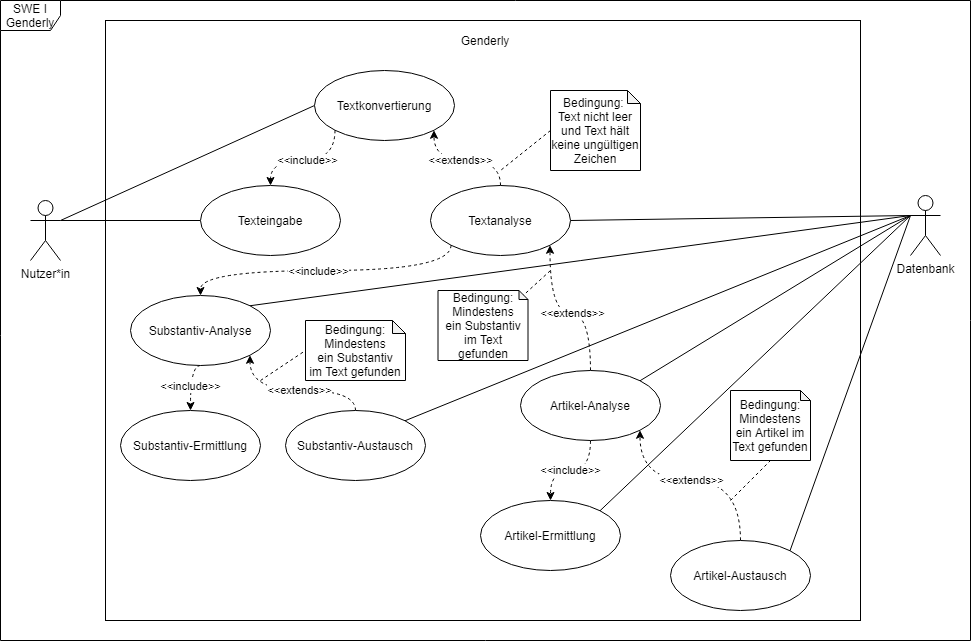
\includegraphics[width=\textwidth]{Bilder/Diagramme/Anwendungsfalldiagramm.png}
\end{adjustbox}
\vspace{0.25cm}

\chapter{Beschreibung}

\vspace{0.25cm}

Gemäß Aufgabenstellung findet die Beschreibung exklusiv unter Anwendung von Use Case-Schablonen zur gesamten Menge der obig gezeigten Use Cases statt.

\vspace{1cm}

\begin{table}[htbp]
\begin{tabular}{|l|l|}
\hline
Name                        & \multicolumn{1}{c|}{\textbf{Texteingabe}} \\ \hline
Kurzbeschreibung            & Nutzer*in gibt Text in dafür vorgesehenes Textfeld ein. \\ \hline
Vorbedingung                & Text ist durch Nutzer*in von Syntaxfehlern bereinigt, in \\
                            & deutscher Sprache und frei von ungültigen Zeichen \\
                            & (wie z.B. Steuerzeichen). \\ \hline
Nachbedingung               & Eingegebener Text wird in Oberfläche angezeigt. \\ \hline
Fehlersituation             & Nutzer*in hat Text mit ungültigen Zeichen eingegeben \\ \hline
Systemzustand im Fehlerfall & Eingegebener Text verworfen, Oberfläche zurückgesetzt, \\
                            & neue Eingabe erwartet. \\ \hline
Akteure                     & Nutzer*in \\ \hline
Trigger                     & Eingabe durch Nutzer*in \\ \hline
Standardablauf              & 1. Aufnahme und Anzeige des eingegebenen Textes, \\
                            & 2. Prüfung auf ungültige Zeichen im Text, \\
                            & 3. Weiterleitung des Textes an den Analyse-Prozess, \\ \hline
Alternativablauf            & 1. Aufnahme und Anzeige des eingegebenen Textes, \\
                            & 2. Prüfung auf ungültige Zeichen im Text, \\
                            & 3. Nutzer*in über ungültige Zeichen benachrichtigen. \\ \hline
\end{tabular}
\end{table}

\begin{table}[htb]
\begin{tabular}{|l|l|}
\hline
Name                        & \multicolumn{1}{c|}{\textbf{Textkonvertierung}} \\ \hline
Kurzbeschreibung            & Text wird auf Verlangen von Nutzer*in (Knopfdruck) \\ 
                            & eingelesen und umgewandelt. \\ \hline
Vorbedingung                & Nutzer*in hat Text eingegeben, Text wurde auf \\
                            & ungültige Zeichen überprüft. \\ \hline
Nachbedingung               & Analysierter und angepasster Text wird \\
                            & Nutzer*in angezeigt. \\ \hline
Fehlersituation             & Text wird nicht durch Nutzer*in eingegeben. \\ \hline
Systemzustand im Fehlerfall & Text wird nicht konvertiert. \\ \hline
Akteure                     & Nutzer*in \\ \hline
Trigger                     & Nutzer*in drückt Knopf auf System-Oberfläche. \\ \hline
Standardablauf              & 1. Text wird auf Wortanzahl überprüft,\\
                            & 2. Text wird an den Textanalyse-Prozess \\ 
                            &    weitergeleitet, \\ 
                            & 3. Ergebnistext wird vom Textanalyse-Prozess bezogen,\\
                            & 4. Ergebnistext wird auf Wortlänge überprüft, \\
                            & 5. Nicht-leerer Ergebnistext wird aufbereitet \\
                            &    und dargestellt. \\ \hline
Alternativablauf            & 1. Text wird auf Wortanzahl überprüft, dabei wird \\
                            &    leere Wortmenge festgestellt, \\
                            & 2. Text wird nicht konvertiert, \\
                            & 3. Kein Text wird ausgegeben, \\
                            & 4. Nachricht über fehlgeschlagene Konvertierung wird \\
                            &    Nutzer*in angezeigt. \\ \hline
\end{tabular}
\end{table}

\begin{table}[htb]
\begin{tabular}{|l|l|}
\hline
Name                        & \multicolumn{1}{c|}{\textbf{Textanalyse}} \\ \hline
Kurzbeschreibung            & Text wird mithilfe der Datenbank auf ersetzbare \\
                            & Wörter durchsucht. \\ \hline
Vorbedingung                & Text ist eingegeben und eingelesen. \\ \hline
Nachbedingung               & Analysierter und bearbeiteter Text wird zur \\
                            & Darstellung weitergeleitet. \\ \hline
Fehlersituation             & Text enthält nur Leerzeichen. \\ \hline
Systemzustand im Fehlerfall & Textanalyse wird übersprungen. \\ \hline
Akteure                     & Datenbank \\ \hline
Trigger                     & Textkonvertierungsprozess wird gestartet \\
                            & (Knopfdruck des Nutzers bzw. der Nutzerin). \\ \hline
Standardablauf              & 1. Text wird auf Wortanzahl überprüft, \\ 
                            & 2. Text wird in Worte aufgeteilt, \\
                            & 3. Worte werden auf Wortart überprüft, \\
                            & 4. Kontext um Substantive wird erfasst, \\
                            & 5. Datenbank wird nach Substitutions-\\
                            &    Substantiven befragt, \\
                            & 6. Substantive ggf. mit Ersatz-\\
                            &    Substantiven austauschen, \\
                            & 7. Kontext ersetzter Substantive auf \\
                            &    Artikel überprüfen, \\
                            & 8. Im Kontext ersetzter Substantive gefundene \\
                            &    Artikel ggf. ersetzen. \\ \hline
Alternativablauf            & 1. Text wird auf Wortanzahl überprüft \\
                            &    (Leerzeichen zählen hier nicht als Worte), \\
                            & 2. Leere Wortmenge veranlasst Abbruch, \\
                            & 3. Rückgabe eines leeren Ergebnistexts als Zeichen \\
                            &    nicht durchgeführter Analyse. \\ \hline
\end{tabular}
\end{table}

\begin{table}[htb]
\begin{tabular}{|l|l|}
\hline
Name                        & \multicolumn{1}{c|}{\textbf{Substantiv-Analyse}} \\ \hline
Kurzbeschreibung            & Herausfiltern und ggf. Ersetzen der Substantive \\
                            & aus dem Eingabetext. \\ \hline
Vorbedingung                & Nicht leerer, syntaktisch korrekter Text liegt \\
                            & als verarbeitete, die Reihenfolge beachtende \\
                            & Wörterliste vor. \\ \hline
Nachbedingung               & Substantive im Text sind durch korrekt gegenderte \\
                            & Substantive ersetzt worden. \\ \hline
Fehlersituation             & Text enthält keine als Substantiv erkennbaren Wörter. \\ \hline
Systemzustand im Fehlerfall & Keine Textbearbeitung vornehmen. \\ \hline
Akteure                     & Datenbank \\ \hline
Trigger                     & Text erfüllt Bedingung, dass er nicht leer ist und \\
                            & keine ungültigen Zeichen enthält. \\ \hline
Standardablauf              & 1. Im als Wörterliste aufgeteilten Satz nach Worten mit \\
                            &    Großbuchstaben am Beginn suchen, \\
                            & 2. Pro gefundenem Substantiv nach vermerkten, korrekt \\
                            &    gegendertem Ersatz-Substantiv suchen, \\
                            & 3. Substantive mit Ersatz-Substantiven substituieren, \\
                            & 4. Substantiv-Austausch in Wörterliste vermerken. \\ \hline
Alternativablauf            & 1. Im als Wörterliste aufgeteilten Satz nach Worten mit \\
                            &    Großbuchstaben am Beginn suchen, \\
                            & 2. Abbruch der Analyse, \\
                            & 3. Nachricht für Nutzer*in über unauffindbare \\
                            &    Substantive anzeigen. \\ \hline
\end{tabular}
\end{table}

\begin{table}[htbp]
\begin{tabular}{|l|l|}
\hline
Name                        & \multicolumn{1}{c|}{\textbf{Substantiv-Ermittlung}} \\ \hline
Kurzbeschreibung            & Aus gegebener, chronologischer Wörterliste sollen die \\
                            & Substantive ermittelt werden. \\ \hline
Vorbedingung                & Nicht-leerer, syntaktisch korrekter Text liegt \\
                            & als verarbeitete, chronologische Wörterliste vor. \\ \hline
Nachbedingung               & Substantive der Wörterliste als solche erkannt und \\
                            & in der Liste vermerkt. \\ \hline
Fehlersituation             & Text enthält keine als Substantiv erkennbaren Wörter. \\ \hline
Systemzustand im Fehlerfall & Keine Vermerke in der Wörterliste vornehmen. \\ \hline
Akteure                     & \small{\textit{Keine externen Akteure}} \\ \hline
Trigger                     & Text erfüllt Bedingung, dass er nicht leer ist und \\
                            & keine ungültigen Zeichen enthält. \\ \hline
Standardablauf              & 1. Im als Wörterliste aufgeteilten Satz nach Worten mit \\
                            &    Großbuchstaben am Beginn suchen, \\
                            & 2. Jeweils bei gefundenen Listeineinträgen einen \\
                            &    Vermerk hinzufügen. \\ \hline
Alternativablauf            & 1. Im als Wörterliste aufgeteilten Satz nach Worten mit \\
                            &    Großbuchstaben am Beginn suchen, \\
                            & 2. Abbruch der Analyse (kein Substantiv gefunden), \\
                            & 3. Keine Vermerke in der Wörterliste tätigen. \\ \hline
\end{tabular}
\end{table}

\newpage
 
\newpage

\begin{table}[htb]
\begin{tabular}{|l|l|}
\hline
Name                        & \multicolumn{1}{c|}{\textbf{Substantiv-Austausch}} \\ \hline
Kurzbeschreibung            & Vermerkte Substantiv-Einträge einer Wörterliste werden \\
                            & mit Inhalten einer Datenbank verglichen und \\
                            & ggf. substituiert. \\ \hline
Vorbedingung                & Eine Wörterliste aus dem Text wurde gebildet, \\
                            & Substantive wurden mit Vermerken versehen. \\ \hline
Nachbedingung               & Vermerkte Substantive der Liste, falls notwendig, \\
                            & um Ersatzwort substituiert und vermerkt. \\ \hline
Fehlersituation             & Wörterliste ohne Vermerke zu gefundenen Substantiven \\
                            & soll verarbeitet werden. \\ \hline
Systemzustand im Fehlerfall & Überspringen der Bearbeitung bzw. Analyse. \\ \hline
Akteure                     & Datenbank \\ \hline
Trigger                     & Substantive der Wörterliste wurden als solche erkannt und \\
                            & in der Liste vermerkt. \\ \hline
Standardablauf              & 1. Wörterliste nach Einträgen mit Vermerken suchen, \\
                            & 2. Pro vermerktem Substantiv wird die Datenbank nach \\ 
                            &    Ersatz befragt, \\
                            & 3. Ersatzwort einfügen bzw. Wort beibehalten, wenn kein \\
                            &    Ersatz nötig, \\
                            & 4. Bearbeitung des Substantivs am Listeneintrag \\
                            &    vermerken.\\ \hline
Alternativablauf            & 1. Wörterliste nach Einträgen mit Vermerken suchen, \\
                            & 2. Menge der gefundenen Vermerke als leer identifizieren. \\ \hline
\end{tabular}
\end{table}

\newpage
 
\newpage
 
\newpage

\begin{table}[hbt!]
\begin{tabular}{|l|l|}
\hline
Name                        & \multicolumn{1}{c|}{\textbf{Artikel-Analyse}} \\ \hline
Kurzbeschreibung            & Herausfiltern und Ersetzen der Wortmenge der Artikel \\
                            & im unmittelbaren Umfeld ersetzter Substantive. \\ \hline
Vorbedingung                & Für eine Wörterliste wurden Substantive bereits \\
                            & analysiert, ggf. substituiert. Die Substitutionen \\
                            & wurden je Substantiv in Liste jeweils vermerkt. \\ \hline
Nachbedingung               & Artikel im Text sind durch korrekt gegenderte \\
                            & Artikel ersetzt worden. \\ \hline
Fehlersituation             & Keines der vermerkten Substantive wurde substituiert. \\ \hline
Systemzustand im Fehlerfall & Keine Textbearbeitung vornehmen. \\ \hline
Akteure                     & Datenbank \\ \hline
Trigger                     & Wörterliste durch Substantiv-Analyse bearbeitet. \\ \hline
Standardablauf              & 1. In bearbeiteter Wörterliste Einträgen mit Vermerk \\
                            &    für Substantiv-Austausch suchen, \\
                            & 2. Ersatz für Vorgänger-Eintrag des Substantiv-Eintrags\\
                            &    suchen und ggf. einfügen, \\
                            & 3. Ersatz für Nachfolger-Eintrag des Substantiv-Eintrags\\
                            &    suchen und ggf. einfügen. \\ \hline
Alternativablauf            & 1. Abbruch der Analyse (kein Artikel-Ersatz nötig), \\
                            & 2. Weiterleitung aktueller Wörterliste zur Darstellung. \\ \hline

\end{tabular}
\end{table}

\newpage
 
\newpage
 
\newpage

\begin{table}[hbt!]
\begin{tabular}{|l|l|}
\hline
Name                        & \multicolumn{1}{c|}{\textbf{Artikel-Ermittlung}} \\ \hline
Kurzbeschreibung            & Aus gegebener, chronologischer Wörterliste werden Artikel \\
                            & um ersetzte Substantive herum gesucht und ggf. ersetzt. \\ \hline
Vorbedingung                & Wörterliste, die Vermerke zu ersetzten Substantiven \\
                            & enthält. \\ \hline
Nachbedingung               & Artikel vor bzw. nach ersetztem Substantiv als solche \\
                            & erkannt und in Wörterliste vermerkt. \\ \hline
Fehlersituation             & Wörterliste enthält keine Vermerke zu ersetzten \\
                            & Substantiven. \\ \hline
Systemzustand im Fehlerfall & Analyse beendet, Wörterliste wird als Ergebnis gezeigt. \\ \hline
Akteure                     & Datenbank \\ \hline
Trigger                     & Wörterliste durch Substantiv-Analyse bearbeitet. \\ \hline
Standardablauf              & 1. In Wörterliste nach als ersetzt vermerkten \\
                            &    Substantiven suchen, \\
                            & 2. Jeweils bei gefundenen Listeineinträgen Vorgänger- \\
                            &    und Nachfolger-Eintrag mit Datenbank-Einträgen \\
                            &    verleichen, \\
                            & 3. Vermerk bei denjenigen Artikeln vornehmen, zu denen \\
                            &    ein Eintrag in der Datenbank existiert. \\ \hline
Alternativablauf            & 1. In Wörterliste nach als ersetzt vermerkten \\
                            &    Substantiven suchen, \\
                            & 2. Keine gefundenen Vermerke als Anlass zum \\
                            &    Analyse-Abbruch nehmen, \\
                            & 3. Wörterliste zwecks Darstellung aufbereiten lassen. \\ \hline
\end{tabular}
\end{table}

\begin{table}[hbt!]
\begin{tabular}{|l|l|}
\hline
Name                        & \multicolumn{1}{c|}{\textbf{Artikel-Austausch}} \\ \hline
Kurzbeschreibung            & Vermerkte Artikel der Wörterliste werden mit Inhalten \\
                            & einer Datenbank verglichen und ggf. substituiert. \\ \hline
Vorbedingung                & Wörterliste, die Vermerke für zu ersetzende Artikel \\
                            & enthält. \\ \hline
Nachbedingung               & Vermerkte Artikel der Liste wurden, falls notwendig, \\
                            & um Ersatzartikel substituiert. \\ \hline
Fehlersituation             & Wörterliste ohne Vermerke zu gefundenen Artikeln \\
                            & soll verarbeitet werden. \\ \hline
Systemzustand im Fehlerfall & Analyse beendet, Wörterliste wird als Ergebnis gezeigt. \\ \hline
Akteure                     & Datenbank \\ \hline
Trigger                     & Artikel der Wörterliste wurden als solche erkannt und \\
                            & in der Liste vermerkt. \\ \hline
Standardablauf              & 1. Wörterliste nach Einträgen mit Vermerken suchen, \\
                            & 2. Pro vermerktem Artikel wird die Datenbank nach \\ 
                            &    Ersatz befragt, \\
                            & 3. Ersatzwort einfügen bzw. Wort beibehalten, wenn kein \\
                            &    Ersatz nötig, \\
                            & 4. Bearbeitung des Artikels am Listeneintrag \\
                            &    vermerken. \\ \hline
Alternativablauf            & 1. Wörterliste nach Einträgen mit Vermerken suchen, \\
                            & 2. Keine gefundenen Artikel-Vermerke als Anlass zum \\
                            &    Analyse-Abbruch nehmen, \\
                            & 3. Wörterliste zwecks Darstellung aufbereiten lassen. \\ \hline 
\end{tabular}
\end{table}

%TC:ignore

%Glossar
\printglossary
\pagebreak

\nocite{*}
%\bibliography{Literatur}
%\bibliographystyle{alphadin}


%\subfile{Anhang/main}
%TC:endignore

\end{document}